\documentclass[10pt,twocolumn]{article}
\usepackage[margin=0.75in]{geometry}
\usepackage[T1]{fontenc}
\usepackage{lmodern,microtype,amsmath,amssymb,booktabs,graphicx,natbib,url}
\usepackage[colorlinks=true,allcolors=blue]{hyperref}
\makeatletter
\g@addto@macro\UrlBreaks{\do\-}
\makeatother
\setlength{\columnsep}{0.25in}
\raggedbottom
\newcommand{\ind}{1}
\title{When Do Relations Help Collective Forecasts?\\A Controlled Study of Operational Temporal Graphs}
\author{Anonymous manuscript for author review}
\date{}
\begin{document}
\maketitle
\begin{abstract}
Individual event probabilities on temporal operational graphs do not determine
the uncertainty of group counts or simultaneous delays. We build a
current-cohort forecasting benchmark on a compute-cluster trace and two
loan-workflow releases, separating marginal prediction, shared dependence,
typed incidence and group-risk evaluation. Controls include temporal neural
and tree predictors, classical factor scenarios, direct count distributions,
historical residuals and discrete probabilistic reconciliation. Original
frozen evaluations motivate explicitly retrospective calibration and graph
diagnostics; a separately frozen workflow period provides fresh confirmation.
Typed factors reduce cluster count CRPS by 24.3\% against independence, but
only 2.2\% beyond a global factor. Recent same-version calibration and direct
count fitting substantially change the workflow comparison. In fresh
confirmation, global dependence improves count CRPS by 12.7\% while worsening
a reserve-loss proxy by 20.4\%; a development-selected direct count model
outperforms it on both. Count and peak-group-delay rankings also differ.
The contribution is a reproducible application benchmark and controlled
empirical evidence for evaluating mean bias, collective uncertainty and
operational risk separately, with explicit limits on temporal replication
and deployment interpretation.
\end{abstract}

\section{Introduction}
A cluster operator sees tasks belonging to jobs and machines; an incident
manager sees unresolved tickets linked to handlers and teams. Both need
collective forecasts: how many current entities
will remain unresolved, and which groups might fall behind together? Temporal
models can supply each entity's event probability, but those probabilities
alone do not specify the distribution of group counts or the largest group
delay. Moreover, a well-scored count distribution need not support the
particular decision quantile used by an operator.

This study asks a practical evaluation question: \emph{what additional evidence
is needed before individual forecasts on a temporal operational graph can be
used as collective scenarios?} Three issues are easily conflated. Individual
predictions may share a mean bias. Outcomes may retain common variation after
conditioning on observed history. Typed relations may identify additional
association beyond a global factor. Improving the first issue, adding the
second, and exploiting the third require different controls. An apparent
``graph benefit'' against independent sampling can otherwise be mostly a
benefit of shared uncertainty available without typed relations.

We define a common current-cohort target for six public logs: a compute-cluster
trace, Azure VMs, two loan-workflow releases, and two IT-incident sources.
At each origin, a timestamp-bounded
adapter reconstructs the active entities and their observed memberships.
Scenarios assign each entity a first-exit bin across four horizons, including
survival beyond the final horizon. The cohort is not selected using future
exits, arrivals or assignments. The resulting counts can be projected onto
overlapping jobs and machines or onto recent-handler groups.

The contribution is a reproducible benchmark and controlled empirical study,
not a new copula architecture. We compare strong individual predictors,
matched-marginal global and typed factors, direct count distributions,
historical residuals, and discrete probabilistic reconciliation. Delayed
calibration controls separate mean error from dependence, and threshold-free
joint scores test whether count accuracy extends to a group-risk profile.
An initial two-log evaluation motivates retrospective diagnostics; a separately
frozen third-log period and three further frozen source periods supply
confirmation. Storage-bounded transportation pilots and incomplete-history
audits are retained as negative or deferred evidence. The manuscript identifies
these stages explicitly rather than pooling development and confirmation.

Three findings organize the study. Shared factors are strong controls, so the
incremental contribution of typed incidence must be measured against them.
Job grouping and IT handler/team incidence add predictive signal in particular
settings, but graph architecture, relation identity, and dependence are not
interchangeable sources of improvement. Calibration can materially change
both collective scores and asymmetric loss,
but transferring residuals across predictor versions is unreliable. Finally,
methods that forecast individual group counts well can rank differently on
the largest standardized group delay. These findings motivate an evaluation
workflow that checks marginal bias, group-count uncertainty, and joint group
risk separately, rather than treating one score as validation of a scenario
generator.

\section{Related work}
\paragraph{Temporal graphs and event generation.}
GraphMixer illustrates strong temporal encoding with simple components
\citep{cong2023}; our Mixer-style survival predictor is an independent
adaptation, not a reproduction of its link-prediction protocol. CEP3 models
community event times \citep{wang2022}, and DG-Gen generates continuous-time
dynamic graphs \citep{hosseini2025}. Their generation targets differ from
conditional first exits of an already active population. We make no numerical
superiority claim over these systems. Such a comparison requires explicit
state initialization, unknown future-count stopping and outcome adapters.

\paragraph{Joint forecasting and reconciliation.}
TACTiS and TACTiS-2 learn flexible multivariate copulas
\citep{drouin2022,ashok2024}; separating learned marginals from spatial copulas
is also established \citep{huk2025}. Our positive-factor Gaussian and
Marshall--Olkin controls \citep{marshall1967} are deliberately restrictive
classical families. Typed current incidence specifies shared randomness for
changing entities; neither that construction nor the marginal--dependence
decomposition is claimed as a new statistical principle.

Probabilistic reconciliation already conditions forecast distributions on
aggregation constraints, including discrete counts \citep{zambon2024}.
We adapt a two-level importance-conditioning step to vectors of first-exit
category counts and compare it with direct Dirichlet--multinomial forecasts
and bottom-up aggregation. This is an established-method comparator, not a
new reconciliation algorithm or an exact reproduction of an entire software
package. Proper multivariate scores complement marginal scores; the limited
dependence sensitivity of energy scores motivates an additional variogram
score \citep{scheuerer2015}.

\paragraph{Operational forecasting.}
RIMS combines learned predictions and intercase simulation
\citep{meneghello2025}, while AgentSimulator models resource interactions
\citep{kirchdorfer2025}. Closely related work initializes business-process
simulation from current states and estimates conditional uncertainty,
including on BPI 2017 \citep{avramenko2026}. Current-state forecasting and
operational uncertainty are therefore established problems. Our empirical
distinction is to hold individual probabilities fixed when testing incidence,
then separately test correction of those probabilities, direct count
alternatives and joint group-risk scores across workflow and compute logs.
Executable workload generation, such as Mimesys \citep{kim2026}, has a
different output contract: our first-exit scenarios do not reproduce full
workloads, future arrivals or repeated process transitions.

\section{Forecast contract and controls}
Let $V_t$ be the entities active after processing all events recorded by origin
$t$, and let $g_r(i,t)$ denote entity $i$'s observed membership in relation type
$r$. For ordered horizons $h_1<\cdots<h_K$, the outcome
$Y_{ik}=\ind\{T_i\leq t+h_k\}$ records the first exit from the current task
state or the first qualifying application resolution. Each forecast draw
assigns one of $K+1$ categories, with the final category indicating survival
beyond $h_K$. This contract does not predict subsequent returns, exact
within-bin times, or outcomes of future arrivals.

An individual predictor supplies monotone CDFs $F_{ik}$. For a current group
$A$, the expected exit count is $\sum_{i\in A}F_{ik}$ under every coupling,
whereas its variance also includes pairwise outcome covariances. Thus a
coupling can change aggregate dispersion and tails but cannot fix a biased
expected count. We exploit this distinction in two separate experiments:
matched-marginal dependence comparisons and controlled marginal correction.

\subsection{Entity-coherent factor scenarios}
For each draw, generate independent standard normal global, relation-group,
and private factors and set
\begin{equation}
 Z_i=a_iZ_0+\sum_r b_{ir}Z_{r,g_r(i,t)}+c_i\epsilon_i,
 \quad a_i^2+\sum_r b_{ir}^2+c_i^2=1.
\end{equation}
Using $U_i=\Phi(Z_i)$ and $Y_{ik}=\ind\{U_i\leq F_{ik}\}$ preserves each
individual CDF and gives ordered horizon outcomes. Shared draws persist across
streamed entity chunks. Missing memberships transfer their squared loading
to private noise. Identities index incidence; no identity embedding or future
assignment is used. The construction handles simultaneous job and machine
membership without a dense entity covariance matrix.

Independent sampling uses only private noise. Global models learn
state-specific global/private weights; typed models add one weight per
observed relation type. The initial study also includes context-dependent
weight offsets and an exponential common-shock family. All weights are
nonnegative, with at least .02 private variance. These families cannot express
arbitrary negative association. We fit them by composite binary pair
likelihood using earlier out-of-sample individual forecasts, random fitting
horizon pairs, and January or original-development checkpoint selection.
Different calibration treatments receive separate dependence fits in the
fresh replication; retrospective BPI 2017 diagnostics retain original weights
to isolate marginal correction.

We permute noise-sharing incidence within current state and half-unit
last-horizon logit-risk bins, retaining true evaluation groups. This preserves
individual probabilities, fitted weights and group sizes within strata.
Additional Borg controls remove job or machine variance and transfer it to
private noise. These sampler interventions assess predictive grouping under a
fitted model, not causal effects of reassigning actual tasks or people.

\subsection{Delayed calibration}
A shared logit intercept preserves horizon order:
\begin{equation}
 F_{ik}^{(\beta)}=\operatorname{logit}^{-1}
 \{\operatorname{logit}(F_{ik})+\beta\}.
\end{equation}
We fit $\beta\in[-2,2]$ by equal-origin, equal-horizon Bernoulli loss with
$10^{-4}\beta^2$ regularization. The static control uses an earlier calibration
window. Rolling correction uses origins in the previous 60 days whose entire
14-day outcome window has matured; fewer than four eligible origins triggers
an expanding-history fallback. Updated labels enter only after maturity.

A retrospective failure motivates an explicit version control: calibration
residuals from earlier separately fitted predictors need not describe the
current predictor's bias. We therefore compare that transfer with history
from the same fitted predictor. This is a practical calibration control,
not a new online-learning algorithm. Static calibration data also selected
the original neural checkpoint/temperature, so its own fit score is not an
independent validation estimate.

\subsection{Direct counts and discrete reconciliation}
For group $A$, average the individual first-exit category probabilities to
obtain $\bar{\pi}_A$. A conditional Dirichlet--multinomial (DM) baseline uses
\begin{equation}
 N_A\sim\operatorname{DM}(|A|,\kappa q_A),\qquad
 q_A=\operatorname{softmax}(\log\bar\pi_A+\delta).
\end{equation}
We fit one concentration and optionally four category offsets (the fifth is
zero) per projection type, with equal-origin and equal-within-origin-group
likelihood weights. Offsets have fixed weak shrinkage. Concentration-only
and bias-adjusted candidates are selected on development count CRPS.
Training uses complete out-of-sample cohorts, never sampled partial group
counts. Every group draw is bounded, integer-valued and ordered across
horizons. Separately drawn overlapping projections need not correspond to a
common entity realization.

For the retrospective original-log analyses we also fit DM on the more recent
development forecasts, matching the fitting window of historical residuals.
Leave-one-origin-out development CRPS selects concentration-only versus
bias-adjusted DM; all development origins then fit the final predictor.
These selection folds can use later development origins and are not online
validation. Exact beta-binomial cumulative-count marginals supply CRPS and
discrete quantiles for this control; joint-profile scores still use sampled
DM trajectories. This stronger comparison avoids attributing an advantage
to dependence when it comes from access to recent same-version errors.

For the workflow hierarchy, include every handler group, plus an unknown
handler group, in a complete partition. Independently sampled bottom count
vectors $N_g$ are reweighted by the population forecast mass
\begin{equation}
 w^{(m)}\ \propto\ p_{\rm pop}\!\left(\sum_gN_g^{(m)}\right).
\end{equation}
This two-level conditioning adaptation \citep{zambon2024} uses 8,192 proposal
draws and resamples 512 coherent group/population trajectories. We report
effective sample sizes and verify its distribution against an enumerated
small example. Bottom-up aggregation without conditioning is a separate
control. Neither count method preserves individual CDFs. The implemented
hierarchy is complete for workflow handlers; it is not a full crossed
job--machine reconciliation implementation. Historical aggregate residual
resampling remains a comparator in the original two logs.

\section{Evaluation}
We score current-state population counts and observed relation groups of at
least five entities. Fair ensemble CRPS \citep{ferro2014} is divided by current
group size, then averaged equally over groups within projection, horizons,
projection types and origins. This weighting is a benchmark convention, not
an inferred organizational utility. Coverage and width of 90\% intervals are
reported separately by projection.

For remaining current-cohort count $R=|A|-C$, the reserve proxy chooses forecast
quantile $b$ at $r/(r+1)$ and scores
\begin{equation}
 \ell_r(b,R)=\{r(R-b)_++(b-R)_+\}/|A|,\quad r\in\{3,9\}.
\end{equation}
It measures a specified quantile tradeoff, not money or realized staffing
savings. CRPS integrates quantile losses \citep{gneiting2007}; improving it
does not guarantee improvement at this particular quantile.

For joint group risk, let $x_g=C_g/|g|$. We use an energy score with
$d(x,y)=\sqrt{G^{-1}\sum_g(x_g-y_g)^2}$ and a power-.5 variogram score
\citep{scheuerer2015}. The latter averages 2,048 outcome-independent ordered
group pairs; subtracting the ensemble variance divided by draw count removes
finite-ensemble bias of its squared moment error. Its estimate can be slightly
negative. We additionally score the distribution of
\begin{equation}
 D_k=\max_g\frac{\mu_{gk}-C_{gk}}
 {\sqrt{1+\sum_{i\in g}F_{ik}(1-F_{ik})}},
 \qquad \mu_{gk}=\sum_{i\in g}F_{ik}.
\end{equation}
This is the largest standardized slow-progress deviation relative to a
fixed reference forecast. Every compared method uses the same reference
$F$, including recalibrated methods. It measures forecast-relative group
risk, not an observed capacity threshold or an organizational SLA.

We average three random seeds within each origin before paired circular
moving-block resampling (10,000 replicates). Borg blocks span one/two days;
BPI 2017 blocks span 14/28 days; the fresh BPI 2012 analysis prespecifies
seven days with fourteen-day sensitivity. Short traces provide few blocks,
so intervals describe these observed periods and offer limited evidence for
other operating regimes. Cases and random seeds are not independent temporal
replications.

\section{Data and evidence stages}
\label{sec:data}
\begin{table*}[t]
\centering\small
\caption{Six scored sources. An origin is a forecasting time, not an independent
organizational replication. New-period experiments are selected after development
pilots; their models are fixed before target preparation and scoring.}
\label{tab:sources}
\begin{tabular}{llllr}
\toprule
Source & Current-cohort target & Observed relations & Evidence stage & Origins\\
\midrule
Borg 2011 & First pending/running state exit & Job, machine & Original frozen period & 28\\
BPI 2017 & First qualifying application milestone & Last handler & Original frozen period & 61\\
BPI 2012 & First approval/decline/cancellation & Last handler & First confirmation & 28\\
Azure V2 & VM deletion & Deployment, subscription & New-period confirmation & 28\\
UCI incidents & First recorded resolution/closure & Handler, team & New-period confirmation & 28\\
BPI 2014 & First Closed activity after Open & Team & New-period confirmation & 28\\
\bottomrule
\end{tabular}
\end{table*}
The sources span two compute providers and several workflow/incident releases
(Table~\ref{tab:sources}). Their horizons and target semantics differ; scores
are compared within source, not pooled into one cross-domain leaderboard.
All features and memberships use recorded events at or before the origin.
Entire outcome windows must mature before their partition ends. Historical
extracts do not establish complete live populations or ingestion availability.

The initial Borg/BPI 2017 study froze 264 assets. Its outcomes motivated
retrospective direct-count, calibration, and joint-risk controls. BPI 2012 then
froze 82 assets before February scoring. The new extension freezes 165 assets
for Azure days 22--28.75, UCI May 1--28, 2016, and BPI 2014 January 1--28,
2014. The latter adds 84 origins without retuning on their scores. These are
internal holdout freezes, not externally preregistered studies.

New-source model fitting, marginal calibration, dependence fitting, development
validation, and confirmation occupy distinct chronological windows. Three-seed
neural/boosted-tree CDF ensembles are selected by earlier calibration Brier;
copulas and direct counts use the same dependence window. Controls include
feature-matched temporal HGB, node-only and global-set networks, typed message
passing, temporal attention, and relation-specific/shuffled graphs. Gaussian
and Student-$t$ couplings retain the selected marginal probabilities. Complete
windows, feature exclusions, model budgets, and source-selection disclosures
appear in Appendix~\ref{app:design}.

Azure retains all released VMs in a deterministic 5\% sample of subscriptions,
not a prefix of arbitrary VM rows. Google 2019 is audited on one shard only;
incomplete trajectories prevent a valid predictive benchmark. BPI change
snapshots lack reliable attribute-version histories. Citi Bike and two airline
geographies are exploratory pilots, not additional confirmation sources.

\section{Results}
\begin{table*}[t]\centering\small
\caption{Count forecasts on original final periods and fresh BPI 2012 confirmation. Lower CRPS and loss are better; nominal coverage is .90. The three factor rows retain the original individual CDFs. Revised controls on Borg/BPI 2017 are retrospective. DM development-fit scores are exact; sampled methods use 512 draws and three seeds. A dash denotes an unimplemented comparison.}\label{tab:counts}
\begin{tabular}{lrrr rrr rrr}\toprule
&\multicolumn{3}{c}{Borg}&\multicolumn{3}{c}{BPI 2017}&\multicolumn{3}{c}{BPI 2012 (fresh)}\\
Method&CRPS&Cov.&Loss$_9$&CRPS&Cov.&Loss$_9$&CRPS&Cov.&Loss$_9$\\\midrule
Independent&0.0342&0.6594&0.1311&0.0501&0.5356&0.1177&0.0716&0.4745&0.1386\\
Global factor&0.0265&0.9797&0.0551&0.0460&0.8897&0.1290&0.0625&0.8562&0.1669\\
Typed factors&0.0259&0.9059&0.0528&0.0465&0.7935&0.1222&0.0653&0.6655&0.1554\\
DM, earlier fit&0.0287&0.9342&0.0744&0.0450&0.9002&0.1287&0.0389&0.9145&0.1125\\
DM, development fit&0.0285&0.9440&0.0693&0.0408&0.9298&0.1140&---&---&---\\
Bottom-up DM&---&---&---&0.0424&0.7749&0.1326&0.0389&0.8289&0.1176\\
Conditioned DM&---&---&---&0.0418&0.7617&0.1319&0.0390&0.8125&0.1198\\
Historical residuals&0.0309&0.8746&0.0840&0.0439&0.8311&0.1258&---&---&---\\
\bottomrule\end{tabular}\end{table*}

\begin{table*}[t]\centering\small
\caption{BPI 2017 controlled same-version correction. Original Gaussian weights are fixed. These are retrospective diagnostics; improved mean calibration does not guarantee a better reserve quantile.}\label{tab:calibration}
\begin{tabular}{llrr rr}\toprule
& &\multicolumn{2}{c}{October development}&\multicolumn{2}{c}{November--December}\\
Correction&Dependence&CRPS&Loss$_9$&CRPS&Loss$_9$\\\midrule
Identity&Independent&0.0433&0.0954&0.0501&0.1176\\
Identity&Global factor&0.0410&0.1195&0.0459&0.1290\\
Identity&Typed factors&0.0411&0.1088&0.0465&0.1222\\
Static&Independent&0.0401&0.0945&0.0469&0.1197\\
Static&Global factor&0.0386&0.1147&0.0435&0.1244\\
Static&Typed factors&0.0383&0.1039&0.0439&0.1188\\
Rolling 60D&Independent&0.0401&0.0947&0.0435&0.1441\\
Rolling 60D&Global factor&0.0385&0.1146&0.0407&0.1182\\
Rolling 60D&Typed factors&0.0382&0.1037&0.0408&0.1199\\
\bottomrule\end{tabular}\end{table*}

\begin{table*}[t]\centering\small
\caption{Joint group-profile scores. ES is RMS-normalized energy score; Peak is CRPS of the maximum standardized slow-progress deviation. Scales differ across datasets. Original-period rows are retrospective; all fresh endpoints were frozen before opening February.}\label{tab:joint}
\begin{tabular}{lrr rr rr}\toprule
&\multicolumn{2}{c}{Borg}&\multicolumn{2}{c}{BPI 2017}&\multicolumn{2}{c}{BPI 2012 (fresh)}\\
Method&ES&Peak&ES&Peak&ES&Peak\\\midrule
Independent&0.0597&15.7604&0.0957&0.4613&0.1058&0.5183\\
Global factor&0.0575&7.5434&0.0942&0.4608&0.1023&0.4790\\
Typed factors&0.0546&4.1726&0.0942&0.6686&0.1015&0.7362\\
DM, earlier fit&0.0543&3.9903&0.0923&0.9984&0.0859&0.3903\\
DM, development fit&0.0544&4.0844&0.0879&0.5343&---&---\\
Bottom-up DM&---&---&0.0879&0.5380&0.0861&0.3907\\
Conditioned DM&---&---&0.0879&0.5539&0.0860&0.3922\\
Rolling correction + global&---&---&0.0880&0.4363&0.0928&0.4882\\
\bottomrule\end{tabular}\end{table*}

\begin{figure*}[t]
\centering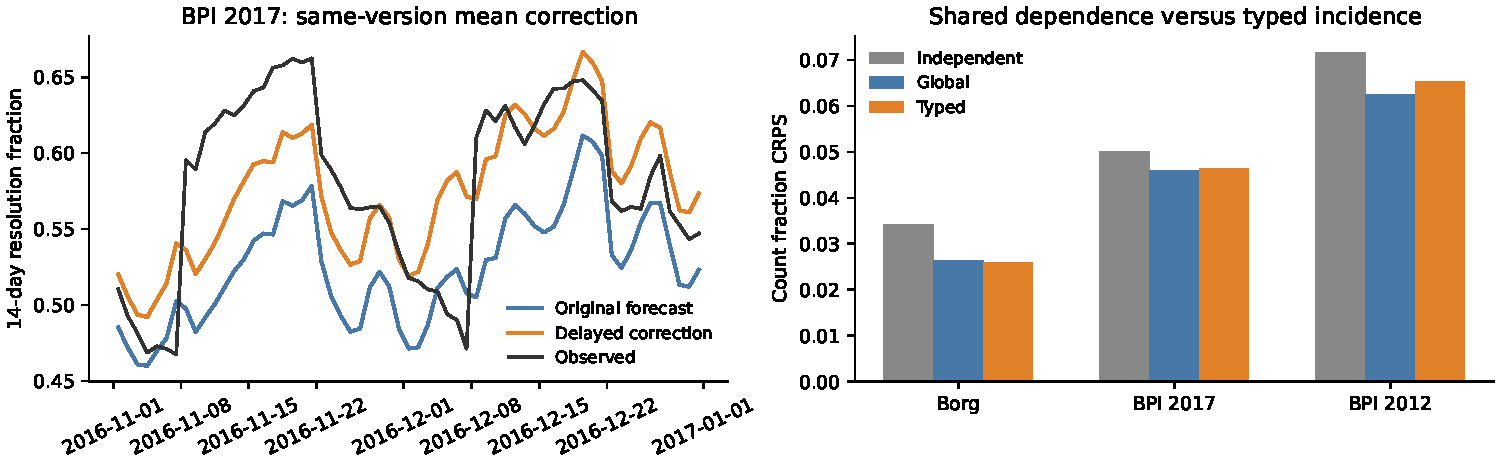
\includegraphics[width=.98\textwidth]{figures/calibration_and_controls.pdf}
\caption{Left: retrospective BPI 2017 fourteen-day population mean predictions
under original and delayed same-version correction. Right: matched-marginal
factor comparisons on original final periods and fresh BPI 2012. The global
factor captures much of the improvement over independence; typed incidence
has an application-specific incremental contribution.}
\label{fig:controls}
\end{figure*}

\subsection{Count gains survive strong controls only in some settings}
The original frozen Borg typed Gaussian model reduces count-fraction CRPS
from .03417 under independence to .02587, a 24.3\% improvement
(Table~\ref{tab:counts}). Ratio-9 reserve loss falls from .13106 to .05280.
The global factor already reaches .02646 CRPS: the additional typed gain is
2.2\%, not 24.3\%. The paired typed-minus-global CRPS interval is
$[-.00105,-.00018]$ with one-day blocks. Removing job variance increases
job-level CRPS from .01451 to .01922; removing machine variance changes
machine CRPS from .02507 to .02525. The strongest demonstrated typed signal
is therefore job grouping, with a much smaller machine contribution.

Stronger direct controls do not remove Borg's count result. The
development-fitted DM model reaches .02853 CRPS and .06931 reserve loss.
Typed-minus-DM CRPS is $-.00266$, with one-day block interval
$[-.00366,-.00169]$. The earlier-OOF DM and historical residual controls are
weaker. Nevertheless, macro coverage is insufficient evidence of uniform
calibration: original typed population coverage is about .763 while job and
machine coverage are about .978 and .976. A macro value near .90 hides this
imbalance.

BPI 2017 gives a different ranking. The original global model improves CRPS
by 8.3\% over independence but increases the reserve loss by 9.6\%.
Development-fitted bias-DM reaches .04077 CRPS and .11396 loss, outperforming
the original global forecast on both. Its CRPS difference is $-.00518$
with 14-day block interval $[-.00983,-.00096]$. Conditioning reconciles
handler/population trajectories but does not improve on the unreconciled
direct count model; its population and group tradeoffs must be inspected
separately. The early-OOF DM is weaker than its same-version development fit,
showing why comparator training windows matter.

\subsection{Calibration changes the operational comparison}
The first retrospective correction transferred June--August OOF errors to
the current BPI 2017 predictor. It made October global-model CRPS worse,
from .04102 to .05422. Those OOF forecasts came from different fitted
predictors. Using earlier September forecasts from the \emph{same} predictor
reverses that failure: delayed correction gives October CRPS .03845.
The later-period global score improves from .04589 to .04072, with paired
difference $-.00517$ and 14-day interval $[-.00859,-.00192]$.
Its fourteen-day mean resolution forecast rises from .525 to .578, against
observed .579. These are controlled follow-ups, not untouched final estimates.

The corrected global model and development-fitted direct DM have almost
identical count CRPS: difference $-.00005$, interval
$[-.00134,.00120]$. Correction therefore does not establish superiority over
a strong direct alternative. Nor is the decision effect uniform. Corrected
global reserve loss falls from .12899 to .11816, whereas corrected
independence worsens from .11761 to .14405. The same improved marginal means
produce different reserve quantiles under different joint laws
(Table~\ref{tab:calibration}). Identity rows here use a common diagnostic
random stream, so they differ slightly from the independently generated
original frozen table.

\subsection{Fresh confirmation favors the direct model}
The February BPI 2012 confirmation was evaluated once under the separately
frozen protocol. The development-selected identity/global model improves
CRPS by 12.7\% over independence (.06253 versus .07162), but worsens
reserve loss by 20.4\% (.16694 versus .13864). Its CRPS difference is
$-.00909$, with seven-day block interval $[-.01081,-.00721]$.
Typed factors are worse than the global control by .00274 CRPS, interval
$[.00187,.00357]$.

The development-selected bias-DM is substantially stronger: .03893 CRPS,
.9145 coverage and .11246 reserve loss. Relative to the selected Gaussian,
CRPS improves 37.7\% and reserve loss 32.6\%; the CRPS-difference interval
is $[-.03183,-.01436]$. Bottom-up and conditioned bias-DM have similar
count CRPS but less favorable coverage and reserve loss. Concentration-only
DM is much weaker, implicating mean correction rather than dispersion alone.

This confirmation is a demanding extrapolation for the individual predictor,
which had only 4,854 training case--origin queries before November. Its
fourteen-day February mean is .468 versus observed .617. Static correction
raises it to .575 and rolling correction to .532; both improve aggregate
CRPS, but neither beats bias-DM. Static correction also outperforms rolling
correction on count CRPS in this period. These outcomes confirm the need for
strong bias/direct-count controls, not universal success of an online update
or a conclusion about the best possible individual model for this source.
Only four seven-day or two fourteen-day blocks are available, limiting the
strength of temporal inference.

\subsection{Joint group risk changes the ranking}
Table~\ref{tab:joint} evaluates full group profiles and the largest standardized
slow-progress deviation. In BPI 2017, recent direct DM improves count CRPS
over the original global model, but its peak-deviation CRPS is worse
(.53433 versus .46081). The paired increase is .07351 with 14-day interval
$[.00348,.14454]$. Thus access to better individual group-count distributions
does not establish better prediction of their joint extreme. Delayed
correction plus global dependence reaches .43633 peak CRPS and .08803
profile energy; typed correction offers no clear general advantage.

Borg's global and typed factors substantially improve peak-deviation scores
over independence, primarily through jobs. Direct DM is also competitive
on joint profiles and peaks, despite weaker count CRPS. In fresh BPI 2012,
bias-DM wins both count and peak-deviation comparisons against the selected
global model (.39031 versus .47902 peak CRPS). There is no universal
coherence-versus-accuracy ranking. Full variogram results and projection-level
scores are released rather than selecting only a favorable multivariate metric.

An earlier simultaneous-alarm endpoint required at least 20\% of groups to
fall more than two reference standard deviations behind. It was absent in
Borg and occurred only once across BPI 2017 final horizon--origin outcomes.
That endpoint is uninformative here and was not promoted as a successful
warning task. Threshold-free profile and peak scores were specified before
opening the fresh period.

\section{Discussion}
\paragraph{An evidence requirement, not a universal winning architecture.}
The benchmark exposes distinctions that an individual-event leaderboard
cannot resolve. A shared factor can improve collective dispersion without
changing a single individual probability. Typed incidence can then add a
smaller, projection-specific gain. Correcting a common bias or forecasting
counts directly can change the ranking again. These are empirical reasons to
include global, direct-count and calibration controls before attributing
collective accuracy to a temporal graph architecture.

\paragraph{Which output is needed?}
If the application asks only for a few fixed group counts, direct count models
are strong and economical candidates. Entity-level factor scenarios supply a
different capability: the same realization can be projected onto overlapping
jobs and machines or an alternative grouping without fitting another count
model. A complete handler hierarchy can also be reconciled coherently. Neither
capability guarantees better prediction. In particular, separate good group
marginals need not give the right extreme across groups, and a globally
coherent scenario can still have biased means or incorrect tails. The joint
profile and peak-deviation scores therefore complement count CRPS.

\paragraph{Calibration and dependence interact.}
Replacing biased individual probabilities changes both expected group counts
and the quantile needed by a reserve proxy. A coupling that improved CRPS
before correction need not have the same decision effect afterward. The
same-version requirement matters because a sequence of chronological OOF
predictors is not one stationary calibration object. Nevertheless, delayed
updates can lag a regime change, and the fresh replication does not justify
claiming that rolling correction always beats a fixed earlier map. A factor
estimated from forecast residuals may absorb misspecification; its value is
predictive rather than evidence of an identified common cause.

\paragraph{Limits of generalization.}
The evidence covers one compute cluster and two workflow releases, with only
seven final Borg days and 28 fresh workflow origins. Four or two bootstrap
blocks in the latter are weak support for long-run uncertainty. Repeated cases,
millions of tasks and Monte Carlo seeds do not multiply independent temporal
replications. Retrospective follow-ups are separated from their motivating
outcomes, and the single fresh confirmation should not be interpreted as
broad external validation. No live operator study, policy deployment, measured
cost saving or resource-capacity ground truth is available.

The benchmark conditions on the currently active cohort and excludes future
arrivals, subsequent exits/returns and membership evolution. Last handler is
an observed association, not exclusive ownership. Positive factor families
cannot represent general negative dependence. A full crossed job--machine
probabilistic reconciliation baseline, adaptations of TACTiS or graph
point-process generators, and complete business-process simulation remain
unimplemented comparisons. The paper makes no superiority claim over them.
The three individual architectures and fixed training budgets are useful
controls, not an exhaustive model search.

\paragraph{Implications for scientific dataset generation.}
A reusable scenario source should declare the conditioning population,
observable history and outcome contract before generating records. It should
also test both individual and collective statistics under meaningful group
projections. Our adapters, score suite and provenance checks provide a bounded
foundation for that purpose. They are not a full synthetic-data factory and
have not been validated by training downstream models on synthetic data.
Extending them requires arrivals, repeated transitions and separate utility
and privacy studies. Original public-source license and attribution terms
remain applicable.

\section{Conclusion}
Across six operational logs, collective forecasting requires evidence beyond
individual-event accuracy. Typed relations add measurable information for
some job, subscription, and incident groups, but a global factor explains much
of the independence gap, and strong direct-count or calibration controls can
erase an apparent advantage. Temporal attention and message passing are useful
comparators, not universal replacements for feature-matched trees. Reliable
evaluation must separate marginal prediction, relation-specific dependence,
and the particular collective decision being scored. Timestamp-bounded
adapters, frozen confirmation assets, negative pilots, and projection-level
scores make those distinctions reproducible while leaving live deployment
and broader temporal replication open.

\bibliographystyle{plainnat}
\bibliography{references}
\appendix
\section{Detailed source and protocol definitions}
\label{app:design}
\subsection{Timestamp-bounded adapters}
\paragraph{Borg.}
All 500 task-event shards of Google ClusterData2011-2 supply the compute
application \citep{google2011}. We replay pending/running states in timestamp
and source order, retaining unknown preceding age for time-zero records.
The target is first state change at 1/5/15/60 minutes, including failures,
evictions and kills as well as completion. Current job and known
running-machine memberships define the graph. The evaluated final prefix
contains 144.6 million events; 28 six-hour origins span elapsed days
22--28.75, with 3,760,001 task--origin queries and 105,077--171,603 active tasks
per origin. Those repeated queries are not independent replications.

\paragraph{BPI 2017.}
The application workflow \citep{vandongen2017} uses first
\texttt{A\_Pending}, \texttt{A\_Denied} or \texttt{A\_Cancelled} after creation
at 1/3/7/14 days. This is a documented application milestone, not repayment
or necessarily the final event. Last observed workflow handling supplies the
relation. We exclude retrospective trace attributes, eventual offer outcomes
and future assignments. The original final period comprises 61 daily noon
UTC origins during November--December 2016, with 114,051 case--origin queries
and 1,484--2,189 cases per cohort.

\paragraph{BPI 2012.}
A fresh workflow release \citep{vandongen2012} supplies an analogous target:
first \texttt{A\_APPROVED}, \texttt{A\_DECLINED} or \texttt{A\_CANCELLED}
after \texttt{A\_SUBMITTED}. We normalize these four activity names only to
reuse the replay adapter, retaining their original target definition. All
other activity names remain distinct; workflow lifecycle values are
normalized to lower case. Missing handlers share no entity-level factor.
This is additional temporal/source evidence, not a claim about another
independent bank. February 1--28, 2012 provides 28 final daily origins, with
23,749 case--origin queries, 793--889 cases per cohort, and
follow-up through March 14 00:00 UTC. Activity vocabulary is derived from
the individual fit prefix only.

In every source, observed events through the origin build features and
memberships; outcomes are attached separately. Entire longest-horizon windows
must be observable. Prefix state carries across date partitions without
revealing future events. Recorded event time is the availability proxy;
the archives do not establish live ingestion latency or exclusive resource
ownership. The municipal BPI 2015 candidate was deferred after a
development-source audit did not establish a sufficiently reliable closure
definition across its activity labels. An Alibaba 2018 task-table candidate
was also deferred: absent end timestamps dominated some reconstructed active
cohorts, and their interpretation as continued running was unverified.
Neither candidate contributed predictive results.

\subsection{Initial frozen evaluation}
The initial study compares HGB personal/global/relational arms and temporal
Mixer, GRU and tabular MLP ensembles. Borg uses 32 base features plus a
144-event-count extension; BPI 2017 uses 103 features. Temporal models use
the last 16 events per task/job/machine or case/handler scope, width 64 and
a five-category first-exit head. Selection uses equal-origin mean Brier over
the four horizons, including monotone calibration variants and three-seed
neural means; no best-seed selection is permitted.

Borg individual training/calibration/development end at days 18/20/22;
dependence uses forward-fold predictions in days 8--10, 12--14 and 16--18,
each produced by earlier fitted and calibrated predictors. BPI 2017 uses
training before September, September calibration and October development,
with June/July/August forward folds for dependence. Selected individual
models are HGB global for pending tasks, HGB relational for running tasks,
and the temperature-calibrated Mixer ensemble for BPI 2017. Gaussian typed
and global models are selected for Borg and BPI respectively.

An immutable 264-file manifest froze code, models and evaluation choices
before those final periods were opened. This was a development-informed
holdout freeze, not external preregistration. A lossless Borg timestamp-type
repair after a replay failure retained all original data and changed no
timestamp value or frozen model. Original scientific results and frozen assets
remain preserved; obsolete manuscript copies are not part of the current paper.

\subsection{Retrospective diagnostics and fresh confirmation}
The initial outcomes motivated the direct DM controls, delayed calibration,
factor removals and joint-profile scores. Their analyses on the original
final periods are therefore \emph{retrospective}. Direct count training uses
24 complete Borg six-hour OOF cohorts and 50 complete BPI 2017 OOF cohorts.
The stronger development-fitted DM control instead uses the eight Borg or
17 BPI 2017 current-version development origins, matching the historical
residual fitting period. Both fitting regimes are retained.
The original residual comparator fits on development residuals,
with leave-one-origin-out development scoring and three sampling seeds.

For fresh confirmation, BPI 2012 individual fitting ends before November 1,
2011; November calibrates the individual model, December fits dependence and
direct counts, and January selects configurations. The global-feature HGB
with identity correction wins individual Brier. Identity/global wins
Gaussian development count CRPS; bias-DM wins the direct comparison;
bias-DM conditioning wins the conditioning comparison. Static and rolling
correction remain prespecified controls, with dependence fitted separately
for each treatment. All six Gaussian fits per seed use only development
data.

Before retaining any February outcomes, a second immutable manifest froze
82 assets, the primary comparisons, metrics, origins and bootstrap settings.
The raw parser had previously discarded every event at or after February 1
before retaining its activity or outcome. Final predictors remain fixed;
only the explicitly prespecified rolling correction may use earlier
February outcomes after their 14-day maturity delay. January 19--31 origins
provide cross-boundary calibration history but are not final score origins.
We retain all prespecified outcomes irrespective of which method wins.
\subsection{Cross-domain extension and stronger graph controls}
We next screened additional public sources with bounded local storage, retaining
unsuccessful and unsuitable candidates. Azure V2 \citep{azure2019} supplies a
second compute provider. A first 49,231-row schema/prediction pilot was followed
by a sample retaining \emph{all released VMs} in subscriptions selected by a
fixed SHA-256 rule (first 32 bits modulo 20 equal zero). The sample is complete
within those released subscriptions, not the provider's full production
population. The target is VM deletion at 5/30/120/360 minutes; observed deployment
and subscription memberships supply two relations. Lifetime CPU summaries,
usage-derived VM categories, and deletion times are excluded from features.
Time-zero creations give an observed age lower bound; timestamp coarsening and
the publisher's workload sampling limit interpretation. The interval adapter
emits creation events only, so Azure temporal tokens summarize prior creations,
not a full stream of VM deletions or CPU measurements.

The UCI incident log \citep{amaral2018} supplies handler and team relations.
We predict the first \emph{recorded} Resolved/Closed update after the first
observed nonterminal update at 1/6/24/72 hours. This is an event-log milestone,
not an estimate of an unobserved physical repair time. Resolution timestamps,
closure codes, eventual resolvers, and SLA outcomes repeated in earlier rows
are excluded. BPI 2014 \citep{vandongen2014activity} supplies timestamped incident
activities and team membership; its target is the first Closed activity after
an observed Open. We do not reconstruct live arrival populations from either
historical case extract. Event timestamps proxy information availability.
Naive incident timestamps are interpreted on a UTC clock for reproducible
partitioning; the archives do not verify operational timezone or ingestion
latency. This convention does not recover daylight-saving transitions.

All sources have distinct individual-fit, calibration, dependence-fit, and
development-validation windows. Entire longest-horizon labels must mature
strictly before each window ends. Azure uses day boundaries 0/10/13/16/20;
UCI uses March 1/22, April 1/15, and May 1, 2016; BPI 2014 uses October 1,
November 1/15, December 1, 2013, and January 1, 2014. Prefix state carries
across boundaries. New-period confirmation fixes 28 origins per source:
Azure days 22--28.75, UCI May 1--28, and BPI 2014 January 1--28.
An executable asset manifest freezes all fitted models and comparisons before
these targets are prepared or scored. Earlier schema audits inspected whole-file
state totals and time ranges; this is an internal prediction-holdout freeze,
not external preregistration or a claim that the raw files were never opened.

\paragraph{Matched individual models.}
Controls include personal-feature HGB, HGB with current relation summaries,
and HGB with the same observed event-history tokens available to temporal
attention. Neural controls use width 48: a node MLP, a global set model,
two rounds of typed entity--group mean message passing, and temporal attention
over the last eight observed relation events followed by message passing.
These are independent survival-target adaptations, not reproductions of TGN,
TGAT, or DyGFormer benchmark systems \citep{rossi2020,xu2020,yu2023}.
Each network uses a five-category first-exit head. UCI trains for 30 epochs;
Azure and BPI 2014 for 20, with AdamW learning rate .001 and weight decay .001.
HGB uses 100 boosting iterations, 15 leaves and L2 penalty 10. Checkpoints and temperature
are chosen on the earlier calibration window; three-seed mean CDFs determine
the selected architecture. Relation-specific and size-preserving shuffled
graph controls keep the input feature set and training budget fixed.
A separate bounded Borg pilot shares the existing 176 engineered features
across models, testing additional message passing beyond those summaries;
its sampled-node scores are not population estimates.

\paragraph{Joint controls.}
Gaussian factors include independent, global, each relation alone,
global-plus-each-relation, combined typed, and shuffled-incidence controls.
Small development-only variance grids and coordinate search fit count scores;
the typed model may reduce to the global control. Coordinate fitting starts
at the global fit and performs two sweeps over weights; it is not an exhaustive
joint-grid optimum. Separately fitted relation-only arms are retained even
when they beat that combined fit. Student-$t$ copulas add a
shared inverse-chi-square scale and compare global and typed variants with
degrees of freedom chosen from 4/8/16. Each draw still uses one entity uniform
across horizons. Concentration-only and bias-adjusted direct DM, exact
beta-binomial count scores, and historical residual forecasts use the same
dependence-fitting period. None is tuned on confirmation.

A small additional comparator uses the unchanged published TACTiS attentional
copula module \citep{drouin2022}, with a custom current-cohort encoder,
randomized discrete probability-integral-transform targets, and rank-adjusted
generated uniforms. All comparators in that pilot use the same 64-node subsets.
It is explicitly a limited adaptation: neither the full time-series model nor
an exact discrete likelihood reproduction, and not evidence of superiority
over TACTiS or TACTiS-2 in their original tasks.

Exploratory fitting uses empirical-ensemble CRPS; confirmation uses the fair
distinct-pair estimator with 512 draws and three sampling seeds. The peak
reference scale in confirmation is $\sqrt{1+\sum_iF_i(1-F_i)}$, as in the
original study. Development pilot peak scores used a max-with-one stabilization
and are not numerically pooled with confirmation. Seeds are averaged within
origin before 2,000 paired circular block replicates with 1/3/7-day blocks.
The same frozen probabilities and reference risk quantities are used for
every joint comparator.

\paragraph{Screened alternatives and limits.}
A Google 2019 \citep{google2019} event-shard audit found approximately 83\% of
sampled entity histories contained one event; that shard cannot support a
complete-trajectory forecast. BPI 2014 change snapshots lack version histories
for planned times and affected configuration items; incident activities offer
a better-supported relation replay. Citi Bike \citep{citibike} and airline
\citep{bts2024} pilots test transportation at small scale. Published trips are
retrospectively filtered, and airline schedule-version availability is an
explicit assumption. Their exploratory scores are not presented as live
deployment results. Source selection followed development feasibility and
performance, so reporting all screened candidates is part of the evidence.


\section{Implementation and reproduction details}
\paragraph{Individual and dependence models.}
The original HGB runs use 250 iterations, 31 leaves, minimum leaf size 100,
learning rate .05 and L2 regularization 1. Neural models use width 64, up to
30 epochs, AdamW at .001, gradient clipping at 5 and calibration-window
early stopping with patience 5. Case/job/machine histories contain at most
16 prior events per scope; time lags are computed at the origin. All initial
neural architectures have three-seed ensembles. The fresh HGB control uses
15 leaves and minimum leaf size 50 because its fit window is smaller; it
does not repeat the full neural architecture search. This difference is a
limitation of the fresh replication, not a claim of universal model optimality.

Pair sampling draws 1,000 uniform entity pairs per origin and, per relation,
1,000 uniformly selected group pairs and 1,000 group-size-weighted pairs.
It never conditions on future labels. Static/global AdamW uses learning rate
.02 and up to 50 epochs, with development pair-likelihood patience 8.
The context model in the initial study uses two width-32 SiLU layers,
bounded logit offsets and shrinkage .01. Gaussian probabilities use
32-point double-precision quadrature. Private variance is at least .02.
The common-shock, context and complete individual-arm results remain in the
original artifact; no consistent context-network advantage was established.

DM fits use $\log\kappa\in[-2,12]$ and four offsets in $[-2,2]$, with
$10^{-3}\|\delta\|^2$ penalty. Two fixed concentration initializations are
optimized with analytic gradients and a converged minimum is retained.
A first finite-difference Borg fit stopped at a line-search failure before
producing scores; its directory and source snapshot are preserved. The
analytic-gradient correction changed the repeated BPI count CRPS by less
than $4\times10^{-6}$. Exact cumulative beta-binomial CRPS is checked against
an enumerated pairwise expectation. Reconciliation uses log-normalized
importance weights; all fitting and sampling functions are independently
checked on small known distributions.

\paragraph{Historical residual comparator.}
For each development origin/group, store the four-dimensional residual
$(C-\mu)/\sqrt{1+\sum_iF_i(1-F_i)}$. Each draw selects one common historical
origin, then size-bin-matched group residual vectors. Counts are clipped,
rounded and monotonized. Development scoring omits its own origin; final
scoring uses all development residuals. It changes group means and does not
enforce agreement between overlapping projections. Contrary to one caption
in the original review PDF, its saved evaluator and result files use seeds
0, 1 and 2, not one seed. The correction affects reporting only.

\paragraph{Interval and Monte Carlo interpretation.}
Seed averaging occurs before temporal block resampling. The original
512-to-1,024-draw sensitivity changes macro CRPS by at most .000122 and
preserves within-family rankings. This does not establish sampling precision
for every newly added peak or variogram score; close differences are not
treated as decisive. Fair variogram estimates use sampled group pairs and
can be slightly negative after finite-ensemble correction. Main tables
separate exact direct-count marginal scores from sampled distributions;
exact discrete quantiles and finite-ensemble quantiles can differ slightly.
Projection/horizon CSVs and paired block-size sensitivities accompany the
reported macro values.

\paragraph{Computation and integrity.}
The experiments use two RTX A6000 GPUs, with CPU replay, HGB and direct-count
fits. Original Borg evaluation of five controls over 28 origins requires
about 245--251 seconds per 512-draw process under concurrent shared-device
execution, with at most .67 GiB allocated PyTorch memory; it excludes replay,
training and individual inference and is not an isolated latency benchmark.
The original 264-file freeze and the fresh 82-file freeze are verified after
evaluation. Original code, results and the immutable review archive remain
intact; new diagnostics and manuscript sources live in separate directories.
The test suite covers causal replay, temporal eligibility, coherent sampling,
known DM moments, exact reconciliation on a small enumerated distribution,
and dependence-sensitive profile scores.

\paragraph{Data and access.}
Raw-source manifests retain checksums and publisher URLs. Google trace
attribution follows its CC-BY-4.0 release; BPI datasets retain the 4TU General
Terms of Use specified in their metadata. The artifact does not relicense
third-party data or software. The reproduction package supplies executable
analysis, fitted parameters and score evidence; large original logs are
acquired through the documented source workflow. Author identities, permanent
public artifact links and any venue-specific disclosure must be finalized by
the researcher before submission. No external submission or release has been
made during this study.

\begin{table*}[t]\centering\small
\caption{BPI 2017 controlled same-version correction. Original Gaussian weights are fixed. These are retrospective diagnostics; improved mean calibration does not guarantee a better reserve quantile.}\label{tab:calibration}
\begin{tabular}{llrr rr}\toprule
& &\multicolumn{2}{c}{October development}&\multicolumn{2}{c}{November--December}\\
Correction&Dependence&CRPS&Loss$_9$&CRPS&Loss$_9$\\\midrule
Identity&Independent&0.0433&0.0954&0.0501&0.1176\\
Identity&Global factor&0.0410&0.1195&0.0459&0.1290\\
Identity&Typed factors&0.0411&0.1088&0.0465&0.1222\\
Static&Independent&0.0401&0.0945&0.0469&0.1197\\
Static&Global factor&0.0386&0.1147&0.0435&0.1244\\
Static&Typed factors&0.0383&0.1039&0.0439&0.1188\\
Rolling 60D&Independent&0.0401&0.0947&0.0435&0.1441\\
Rolling 60D&Global factor&0.0385&0.1146&0.0407&0.1182\\
Rolling 60D&Typed factors&0.0382&0.1037&0.0408&0.1199\\
\bottomrule\end{tabular}\end{table*}

\begin{table*}[t]\centering\small
\caption{Joint group-profile scores. ES is RMS-normalized energy score; Peak is CRPS of the maximum standardized slow-progress deviation. Scales differ across datasets. Original-period rows are retrospective; all fresh endpoints were frozen before opening February.}\label{tab:joint}
\begin{tabular}{lrr rr rr}\toprule
&\multicolumn{2}{c}{Borg}&\multicolumn{2}{c}{BPI 2017}&\multicolumn{2}{c}{BPI 2012 (fresh)}\\
Method&ES&Peak&ES&Peak&ES&Peak\\\midrule
Independent&0.0597&15.7604&0.0957&0.4613&0.1058&0.5183\\
Global factor&0.0575&7.5434&0.0942&0.4608&0.1023&0.4790\\
Typed factors&0.0546&4.1726&0.0942&0.6686&0.1015&0.7362\\
DM, earlier fit&0.0543&3.9903&0.0923&0.9984&0.0859&0.3903\\
DM, development fit&0.0544&4.0844&0.0879&0.5343&---&---\\
Bottom-up DM&---&---&0.0879&0.5380&0.0861&0.3907\\
Conditioned DM&---&---&0.0879&0.5539&0.0860&0.3922\\
Rolling correction + global&---&---&0.0880&0.4363&0.0928&0.4882\\
\bottomrule\end{tabular}\end{table*}

\begin{figure*}[t]
\centering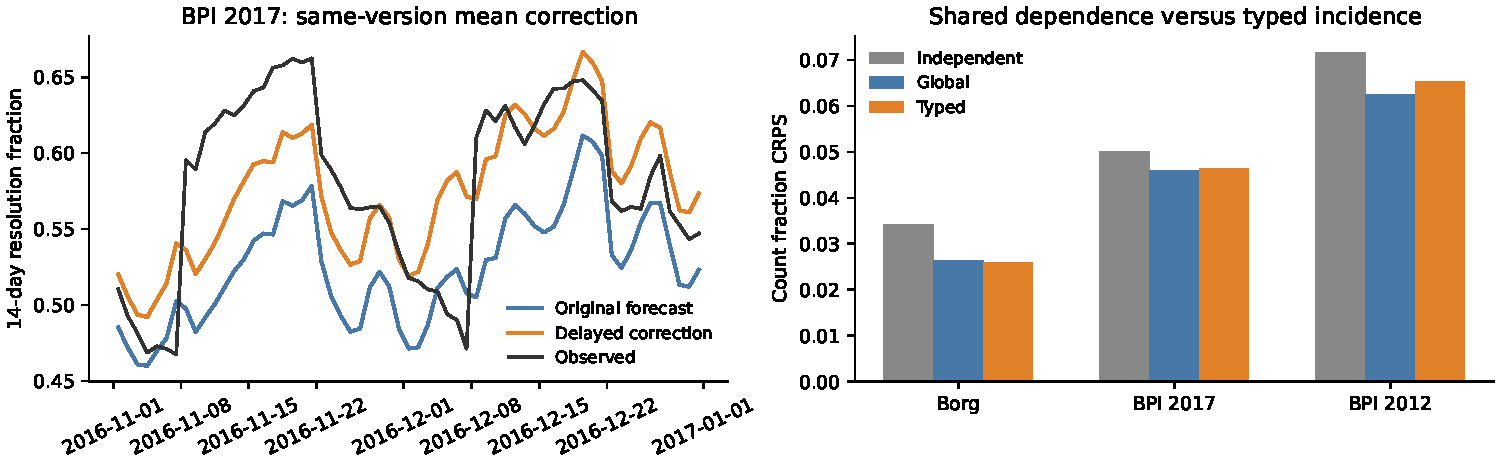
\includegraphics[width=.98\textwidth]{figures/calibration_and_controls.pdf}
\caption{Retrospective BPI 2017 fourteen-day population forecasts under original
and delayed same-version correction (left); matched-marginal factor comparisons
on original final periods and fresh BPI 2012 (right). Global dependence captures
much of the independence improvement; typed incidence adds a smaller,
application-specific contribution.}
\label{fig:controls}
\end{figure*}
\begin{table*}[t]
\centering\small
\caption{All-source confirmation distribution diagnostics. Coverage targets .90; width is in cohort fractions. Energy, fair variogram and peak-deviation CRPS are lower-is-better. Direct DM joint profiles are separately generated group trajectories, not coherent entity-level realizations.}\label{tab:extension-joint}
\begin{tabular}{llrrrrr}
\toprule
Source & Model & Cov. & Width & Energy & Variogram & Peak \\
\midrule
UCI incidents & Independent & 0.669 & 0.144 & 0.06817 & 0.02670 & 1.791 \\
UCI incidents & Gaussian global & 0.908 & 0.236 & 0.06524 & 0.02689 & 1.396 \\
UCI incidents & Gaussian typed & 0.847 & 0.263 & 0.06433 & 0.02568 & 1.107 \\
UCI incidents & Student-$t$ global & 0.937 & 0.247 & 0.06536 & 0.02692 & 1.381 \\
UCI incidents & Student-$t$ typed & 0.922 & 0.277 & 0.06371 & 0.02563 & 1.054 \\
UCI incidents & Direct DM & 0.931 & 0.241 & 0.06411 & 0.02544 & 1.094 \\
UCI incidents & Bias-DM & 0.935 & 0.269 & 0.06366 & 0.02613 & 1.069 \\
Azure V2 & Independent & 0.765 & 0.022 & 0.03744 & 0.01045 & 2.698 \\
Azure V2 & Gaussian global & 0.985 & 0.041 & 0.03720 & 0.01018 & 2.178 \\
Azure V2 & Gaussian typed & 0.985 & 0.041 & 0.03720 & 0.01018 & 2.178 \\
Azure V2 & Student-$t$ global & 0.981 & 0.040 & 0.03716 & 0.01023 & 2.165 \\
Azure V2 & Student-$t$ typed & 0.981 & 0.040 & 0.03716 & 0.01023 & 2.165 \\
Azure V2 & Direct DM & 0.950 & 0.033 & 0.03446 & 0.01006 & 1.650 \\
Azure V2 & Bias-DM & 0.948 & 0.031 & 0.03439 & 0.00986 & 1.629 \\
BPI 2014 & Independent & 0.693 & 0.118 & 0.04777 & 0.01505 & 1.349 \\
BPI 2014 & Gaussian global & 0.915 & 0.166 & 0.04736 & 0.01520 & 1.237 \\
BPI 2014 & Gaussian typed & 0.927 & 0.177 & 0.04718 & 0.01506 & 1.211 \\
BPI 2014 & Student-$t$ global & 0.948 & 0.178 & 0.04776 & 0.01534 & 1.250 \\
BPI 2014 & Student-$t$ typed & 0.955 & 0.189 & 0.04761 & 0.01520 & 1.240 \\
BPI 2014 & Direct DM & 0.915 & 0.166 & 0.04658 & 0.01488 & 1.174 \\
BPI 2014 & Bias-DM & 0.848 & 0.155 & 0.04906 & 0.01503 & 1.411 \\
\bottomrule
\end{tabular}
\end{table*}

\begin{table*}[t]
\centering\small
\caption{Frozen relation controls. Variance weights are global/handler/team (UCI), global/deployment/subscription (Azure), and global/team (BPI14). Only degrees of freedom change between matched Gaussian and Student-$t$ arms; Student-$t$ uses a shared scale. Scores are $\times 1,000$.}\label{tab:extension-relations}
\begin{tabular}{lllrrr}
\toprule
Source & Coupling & Weights & $\nu$ & CRPS & Loss \\
\midrule
UCI incidents & G: global & 0.15/0/0 & --- & 44.57 & 92.39 \\
UCI incidents & G: handler & 0/0.5/0 & --- & 44.49 & 105.93 \\
UCI incidents & G: global handler & 0.15/0.15/0 & --- & 43.82 & 86.52 \\
UCI incidents & G: team & 0/0/0.3 & --- & 43.67 & 95.06 \\
UCI incidents & G: global team & 0.15/0/0.15 & --- & 43.59 & 84.56 \\
UCI incidents & G: typed & 0/0.3/0.3 & --- & 43.11 & 90.42 \\
UCI incidents & $t$: global & 0.15/0/0 & 16 & 44.44 & 91.18 \\
UCI incidents & $t$: typed & 0/0.3/0.3 & 16 & 42.84 & 84.72 \\
Azure V2 & G: global & 0.7/0/0 & --- & 7.60 & 14.20 \\
Azure V2 & G: deployment & 0/0.7/0 & --- & 7.28 & 13.09 \\
Azure V2 & G: global deployment & 0.7/0/0 & --- & 7.60 & 14.20 \\
Azure V2 & G: subscription & 0/0/0.7 & --- & 7.25 & 13.00 \\
Azure V2 & G: global subscription & 0.7/0/0 & --- & 7.60 & 14.20 \\
Azure V2 & G: typed & 0.7/0/0 & --- & 7.60 & 14.20 \\
Azure V2 & $t$: global & 0.7/0/0 & 4 & 7.58 & 14.17 \\
Azure V2 & $t$: typed & 0.7/0/0 & 4 & 7.58 & 14.17 \\
BPI 2014 & G: global & 0.05/0 & --- & 34.15 & 85.89 \\
BPI 2014 & G: team & 0/0.15 & --- & 33.74 & 78.76 \\
BPI 2014 & G: global team & 0.05/0.05 & --- & 34.08 & 86.14 \\
BPI 2014 & G: typed & 0.05/0.05 & --- & 34.08 & 86.14 \\
BPI 2014 & $t$: global & 0.05/0 & 16 & 34.41 & 87.91 \\
BPI 2014 & $t$: typed & 0.05/0.05 & 16 & 34.40 & 88.25 \\
\bottomrule
\end{tabular}
\end{table*}

\end{document}
